\documentclass[preprint,12pt]{elsarticle}

\usepackage{graphicx}
\usepackage{amsmath,amssymb}
\usepackage{booktabs}
\usepackage{multirow}
\usepackage{url}
\usepackage{xcolor}
\usepackage{array}
\usepackage{caption}
\usepackage{subcaption}
\usepackage[section]{placeins}

\journal{Image and Vision Computing}
\biboptions{sort&compress}
\renewcommand{\topfraction}{0.9}
\renewcommand{\textfraction}{0.05}
\renewcommand{\floatpagefraction}{0.85}
\setlength{\textfloatsep}{10pt plus 2pt minus 2pt}
\setlength{\floatsep}{8pt plus 2pt minus 2pt}
\setlength{\intextsep}{8pt plus 2pt minus 2pt}
\setlength{\abovecaptionskip}{4pt}
\setlength{\belowcaptionskip}{2pt}
\setlength{\emergencystretch}{1.5em}
\captionsetup{font=small,labelfont=bf}
\captionsetup[subfigure]{font=footnotesize,labelfont=bf}
\raggedbottom

\begin{document}

\begin{frontmatter}

\title{GRA-CNN: Semantic-Aware Structured Channel Pruning via Gray Relational Analysis}

\author[label1]{Kangrui Li}
\author[label1]{Junyi Lin}
\author[label1]{Xiaobo Zhang\corref{cor1}}
\ead{zxb_leng@gdut.edu.cn}

\cortext[cor1]{Corresponding author.}
\affiliation[label1]{
  organization={Faculty of Automation, Guangdong University of Technology},
  city={Guangzhou},
  country={China}
}

\begin{abstract}
Structured channel pruning is widely used to compress convolutional networks for practical vision deployment, yet most pruning criteria are driven by local structural cues and do not test whether a channel is semantically redundant across class-specific activation patterns. We present GRA-CNN, a semantic-aware structured pruning framework that combines a structural anchor based on channel independence, Taylor sensitivity, and Fisher information with a quality-gated boundary refinement based on Gray Relational Analysis (GRA). The GRA branch estimates class-aware inter-channel redundancy and is activated only in layers where the semantic signal is sufficiently reliable. As a result, semantic scoring acts as a targeted correction near the keep/prune boundary rather than a full replacement for structural ranking. We evaluate the method on ResNet-56 and VGG-16 on CIFAR-100, a five-ratio transfer sweep on ResNet-18/Tiny-ImageNet, strict equal-budget comparisons, multi-seed component ablations, and device-level latency profiling. The results show a consistent advantage over CHIP in high-compression residual settings on ResNet-56, while VGG-16 shows a more mixed, architecture-dependent pattern. The ablation study shows that channel attention, boundary refinement, and quality gating all contribute, with the largest penalties appearing at aggressive compression. Overall, GRA-CNN is best viewed as a robustness-oriented semantic refinement for structured pruning: it is most useful when structural-only rankings become brittle, rather than a universally dominant score across all architectures and compression levels.
\end{abstract}

\begin{keyword}
Structured channel pruning \sep Semantic-aware pruning \sep Gray relational analysis \sep Model compression \sep Robust deep learning
\end{keyword}

\end{frontmatter}

\section{Introduction}
\label{sec:introduction}

Convolutional neural networks remain important backbones for visual recognition, but their deployment on resource-constrained devices still depends heavily on model compression. Structured channel pruning is attractive because it removes whole filters, preserves dense tensor layouts, and can therefore translate to practical acceleration without sparse-kernel support~\cite{he2017channel,liu2017network_slimming}. Unlike unstructured pruning, which produces irregular sparsity patterns that require specialized hardware or software support, structured pruning maintains compatibility with standard deep learning frameworks and inference engines. The central difficulty is no longer whether channels can be removed, but how to decide \emph{which} channels are genuinely dispensable for the final visual decision without sacrificing accuracy or introducing instability across different compression ratios and random initializations.

Most structured pruning criteria still rely on local structural heuristics. Magnitude-based methods remove filters with small norms~\cite{li2017pruning}, while Taylor-based criteria approximate the loss increase caused by channel removal~\cite{molchanov2019taylor}. Geometric approaches such as FPGM remove filters near the layer manifold center~\cite{he2019fpgm}, and rank-based methods such as HRank exploit low-rank feature maps~\cite{lin2020hrank}. These criteria are computationally efficient and often competitive in moderate compression regimes, but they do not explicitly test whether a channel is semantically redundant across classes. A channel may look weak in magnitude or geometry while still preserving class-discriminative response trends that are hard to replace once compression becomes aggressive, particularly in deep networks where feature representations become increasingly abstract and task-specific.

We address this gap through \textbf{GRA-CNN}, a structured pruning framework that uses \textbf{Gray Relational Analysis (GRA)} to model class-aware semantic redundancy. Rather than replacing structural scoring outright, GRA-CNN uses a two-stage design. A structural anchor first provides a stable global ranking based on channel independence, Taylor sensitivity, and Fisher information, and a quality-gated semantic branch then refines channels only near the keep/prune boundary when the redundancy signal is reliable. This design reflects a practical viewpoint: semantic scoring is most useful as a correction in stressed regimes, especially when structural-only rankings begin to lose robustness under aggressive compression.

The study is organized around robustness rather than universal dominance. Across the multi-seed CIFAR-100 experiments, equal-budget comparisons, component ablations, and the five-ratio Tiny-ImageNet transfer sweep, the clearest gains appear in high-compression residual settings. In architecture-sensitive cases, especially plain VGG-style networks, the method is better interpreted as a competitive semantic complement. It is not presented as a uniformly best pruning score.

Our contributions are fourfold:
\begin{itemize}
    \item We introduce a class-aware semantic redundancy score based on Gray Relational Analysis for structured channel pruning.
    \item We design a two-stage pruning strategy that couples a structural anchor with quality-gated boundary refinement.
    \item We conduct a controlled evaluation with multi-seed paired statistics, matched-budget comparisons, and a similarity-metric sensitivity study that separates the framework contribution from the specific choice of GRA.
    \item We provide cross-dataset, multi-compression validation together with supplementary runtime and deployment diagnostics.
\end{itemize}

\section{Related Work}
\label{sec:related}

\subsection{Structured channel pruning criteria}

Classical structured pruning methods score channels with local structural signals. Magnitude-based pruning uses filter norms~\cite{li2017pruning}, while network slimming exploits BatchNorm scaling factors~\cite{liu2017network_slimming,ioffe2015batch}. Taylor-based criteria estimate the loss change induced by channel removal~\cite{molchanov2019taylor,molchanov2017variational}, FPGM uses geometric median distance~\cite{he2019fpgm}, and HRank removes channels that produce low-rank activations~\cite{lin2020hrank}. More recent work has explored attention-based importance scoring and gradient-based sensitivity analysis. These methods form strong practical baselines and are computationally efficient, but their signals remain primarily local and do not explicitly model class-aware redundancy. The key limitation is that structural heuristics may discard channels that preserve subtle but critical class-discriminative patterns, especially under aggressive compression.

\subsection{Global pruning, dependencies, and budget control}

Recent work has emphasized global selection, dependency management, and deployment-aware objectives. Representative examples include AMC, MetaPruning, AutoSlim, and EagleEye~\cite{he2018amc,liu2019metapruning,yu2020autoslim,li2020eagleeye}. These methods use reinforcement learning or evolutionary search to optimize layer-wise pruning ratios jointly across the network. DepGraph and its isomorphic extension formalize dependency-safe structural pruning for modern architectures with skip connections and grouped convolutions~\cite{fang2023depgraph,fang2024isomorphic}. Equal-budget and latency-aware formulations further stress that pruning quality should be judged under matched computational budgets, rather than raw nominal ratios alone~\cite{shen2022halp}. This line of work has significantly improved the fairness of pruning comparisons and enabled practical deployment, but the underlying channel scoring functions still rely primarily on structural heuristics and do not directly address class-aware redundancy at the channel level.

\subsection{Semantic and information-aware pruning signals}

Several methods move closer to task-aware channel selection. CHIP uses channel independence to preserve diversity~\cite{sui2021chip}. Information-theoretic approaches such as HSIC-Lasso based pruning relate channel selection to task-relevant information preservation~\cite{guo2023apib}. Group sparsity and regularization-based methods also encode more structured priors during training~\cite{wen2016learning,wang2021greg}. Recent work has explored mutual information maximization and attention-guided pruning to retain task-critical features. Knowledge distillation has also been combined with pruning to preserve semantic representations from teacher networks. However, most of these methods either require expensive retraining or do not explicitly model class-conditioned redundancy at the channel level. This line of work motivates our semantic branch: the key question is not merely whether a channel is weak, but whether its response pattern is redundant with respect to class-conditioned behavior across all classes in the dataset.

\subsection{Gray relational analysis in learning systems}

Gray Relational Analysis is a trend-similarity tool from grey system theory that remains effective under incomplete or noisy observations~\cite{deng1989gra,kuo2008use}. Its scale-invariant sequence comparison has been used in feature selection and other learning-related settings where robust relational scoring is preferable to direct probabilistic modeling~\cite{pal2021gra_histology}. We adapt GRA to structured pruning by measuring whether a channel's activation sequence is redundant relative to other channels \emph{within each class partition}. This produces a class-aware semantic score that complements structural ranking.

\subsection{Pruning for vision tasks and deployment}

Structured pruning has been extensively studied for convolutional networks on image classification benchmarks such as CIFAR and ImageNet. Recent work has extended pruning to object detection, semantic segmentation, and video understanding tasks, where the trade-off between accuracy and efficiency becomes more critical due to higher computational demands. Deployment-oriented studies have also emphasized the gap between theoretical FLOPs reduction and actual latency improvement on target hardware, leading to hardware-aware pruning methods that optimize for specific accelerators or mobile processors. While these advances improve practical applicability, the core channel selection criteria remain largely architecture-agnostic and do not explicitly account for task-specific semantic redundancy patterns that may vary across different visual recognition problems.

\section{Method}
\label{sec:method}

\subsection{Problem setting and notation}

Let $\mathcal{M}$ be a pre-trained CNN with $L$ convolutional layers. Layer $L_k$ contains $C_k$ output channels. A calibration set $\mathcal{D}_B=\{(\mathbf{x}_i,y_i)\}_{i=1}^{B}$ is drawn from the training split and used only for scoring. The calibration set is kept fixed across all pruning iterations to ensure reproducibility and fair comparison. For channel $c$ in layer $L_k$, we denote global-average-pooled activations by $\mathbf{a}_c\in\mathbb{R}^{B}$, channel independence by $I_c$, Taylor sensitivity by $T_c$, Fisher information by $F_c$, semantic importance by $s_c$, and fused structural anchor score by $A_c$. The target pruning ratio is $p\in(0,1)$, representing the fraction of channels to be removed from each layer. The notation $\hat{\cdot}$ denotes min-max normalization within the layer to ensure all scores are on a comparable scale before fusion.

\subsection{Class-aware semantic redundancy via GRA}

The semantic branch is based on a simple intuition: a channel is dispensable only if its activation trend is redundant relative to other channels \emph{for every class}, not merely on average over the dataset. This class-conditioned view is critical because a channel may appear redundant globally while still preserving distinctive patterns for minority classes or hard-to-classify samples. For class $k$, let $\mathbf{p}_c^{(k)}\in\mathbb{R}^{n_k}$ denote the min-max normalized activation sequence of channel $c$ over the $n_k$ calibration samples from class $k$. We choose Gray Relational Analysis over correlation-based or distance-based similarity measures because GRA is robust to scale differences and does not assume linear relationships between channel activations. The Gray relational coefficient between channels $c$ and $j$ for sample index $i$ is
\begin{equation}
\xi_{c,j}^{(k)}(i)=
\frac{\Delta_{\min}^{(k)}+\rho\Delta_{\max}^{(k)}}
{\left|p_c^{(k)}(i)-p_j^{(k)}(i)\right|+\rho\Delta_{\max}^{(k)}},
\label{eq:ivc_gra_coeff}
\end{equation}
where $\rho\in(0,1)$ is the distinguishing coefficient that controls the sensitivity to extreme deviations, and $\Delta_{\min}^{(k)}$, $\Delta_{\max}^{(k)}$ are the class-wise extrema of channel-pair deviations.

The per-class redundancy score is then
\begin{equation}
R_c^{(k)}=\frac{1}{C_k-1}\sum_{j\neq c}\frac{1}{n_k}\sum_{i=1}^{n_k}\xi_{c,j}^{(k)}(i).
\label{eq:ivc_class_redundancy}
\end{equation}
To preserve channels that remain distinctive for at least one class, we use a conservative minimum aggregation,
\begin{equation}
R_c^{\mathrm{CA}}=\min_k R_c^{(k)},
\label{eq:ivc_ca_redundancy}
\end{equation}
and convert redundancy into semantic importance:
\begin{equation}
s_c = 1 - R_c^{\mathrm{CA}}.
\label{eq:ivc_semantic_importance}
\end{equation}
Large $s_c$ values indicate channels whose class-conditional behavior is not easily replaced by neighboring channels.

Here, ``semantic'' denotes a class-conditioned redundancy proxy derived from activation trends, rather than a claim of full semantic interpretation.

\subsection{Structural anchor and boundary refinement}

GRA-CNN does not replace structural ranking globally. Instead, it first forms a structural anchor
\begin{equation}
A_c = w_I \hat{I}_c + w_T \hat{T}_c + w_F \hat{F}_c,
\label{eq:ivc_anchor}
\end{equation}
with weights $w_I=0.60$, $w_T=0.25$, and $w_F=0.15$. The three signals are: channel independence~\cite{sui2021chip}, Taylor sensitivity~\cite{molchanov2019taylor}, and a class-balanced empirical Fisher proxy
\begin{equation}
F_c=\frac{1}{B}\sum_{i=1}^{B} w_{y_i}
\left(\frac{\partial \ell_i}{\partial a_{c,i}} a_{c,i}\right)^2,
\label{eq:ivc_fisher}
\end{equation}
where $w_{y_i}$ is the inverse-frequency class weight inside the calibration split. The weight allocation prioritizes independence because it captures inter-channel diversity without requiring gradient computation, while Taylor and Fisher provide complementary sensitivity signals. This fusion strategy balances computational efficiency with robustness to noisy gradients.

Semantic refinement is restricted to channels near the keep/prune boundary. A layer-specific quality score
\begin{equation}
Q=0.45R+0.35(1-U)+0.20C
\label{eq:ivc_quality}
\end{equation}
combines three diagnostics: anchor-semantic agreement $R = 1 - \mathrm{mean}(|A-s|)$, semantic dispersion $U = \mathrm{std}(s)$, and semantic contrast $C = P_{90}(s) - P_{10}(s)$. The candidate gate threshold is $\tau_c=\max(0.58, P_{70}(Q))$ across prunable layers. If fewer than 40\% of layers satisfy $Q \geq \tau_c$, the threshold is relaxed to $\tau=P_{55}(Q)$; otherwise $\tau=\tau_c$. In gated layers, the keep count is constrained by the target ratio with a minimum keep floor of $\max(4,\lceil 0.1C_k\rceil)$ to avoid degenerate small layers. The boundary band width is $w_{\mathrm{band}}=\max(2,\mathrm{round}((q_{\mathrm{high}}-q_{\mathrm{low}})C_k))$, with $(q_{\mathrm{low}},q_{\mathrm{high}})=(0.40,0.60)$ for $p\geq0.7$ and $(0.35,0.65)$ otherwise. A swap is accepted when $s_{\mathrm{in}}-s_{\mathrm{out}}\geq \theta_s$ and $A_{\mathrm{out}}-A_{\mathrm{in}}\leq \theta_a$, with defaults $\theta_s=0.08$ and $\theta_a=0.06$; a conservative fallback $(0.03,0.08)$ is used only when the strict rule yields no swap. These defaults are fixed for all experiments in this manuscript. In practice, this turns GRA into a targeted correction mechanism instead of a brittle end-to-end scorer.

\subsection{Computational overhead}

The GRA branch adds pairwise channel comparison within each class partition. For a layer with $C$ channels and $B_k$ samples in class $k$, the redundancy computation scales as $O(C^2B_k)$ for the class and $O(C^2B)$ across classes. Empirically, the additional scoring cost remains modest relative to fine-tuning and is substantially smaller than the overall retraining budget. The full scoring-time profile is reported in the Supplementary Material.

\section{Experimental Setup}
\label{sec:experimental_setup}

\subsection{Datasets, architectures, and baselines}

The primary evaluation uses CIFAR-100 with two architectures that expose different pruning behavior: ResNet-56 and VGG-16~\cite{he2016deep,simonyan2014very}. CIFAR-100 contains 50,000 training images and 10,000 test images across 100 classes, with each image at 32×32 resolution. To test transfer beyond CIFAR-scale resolution and class count, we additionally evaluate ResNet-18 on Tiny-ImageNet~\cite{russakovsky2015imagenet}, which contains 100,000 training images and 10,000 validation images across 200 classes at 64×64 resolution. We compare against five widely used pruning baselines: CHIP~\cite{sui2021chip}, L1-Norm~\cite{li2017pruning}, Taylor~\cite{molchanov2019taylor}, FPGM~\cite{he2019fpgm}, and HRank~\cite{lin2020hrank}. These baselines represent diverse pruning philosophies including magnitude-based, gradient-based, geometric, and rank-based criteria.

\subsection{Protocol}

The main paper emphasizes the CIFAR-100 operating points $p=0.7$ and $p=0.9$. The Supplementary Material reports the full five-ratio matrix with $p\in\{0.5,0.6,0.7,0.8,0.9\}$, and ResNet-56 additionally includes paired residual-trend diagnostics at $p=0.8$. The Tiny-ImageNet transfer study uses the same five-ratio sweep on ResNet-18. All reported cells use five seeds $\{42,123,456,789,1024\}$ to ensure reproducibility and statistical reliability. Fine-tuning uses SGD with momentum 0.9, weight decay $5\times 10^{-4}$, initial learning rate 0.01, and cosine annealing over 30 epochs. The batch size is 128 for all experiments. The GRA distinguishing coefficient is fixed at $\rho=0.5$, and scoring uses eight mini-batches of 128 images with class-balanced sampling to ensure each class is adequately represented in the calibration set.

All methods share the same dependency-safe structural projector and the same target retention ratio inside each architecture-ratio cell. Consequently, compression ratio and parameter reduction are method-invariant within a fixed cell and can be reported once alongside the method scores. Baseline implementations follow their original papers with publicly available reference code where applicable.

\subsection{Statistics}

For each cell, we report mean Top-1 accuracy and standard deviation over five seeds. Paired comparisons use strictly matched architecture-ratio-seed tuples to ensure fair statistical inference. We report paired mean deltas, 95\% bootstrap confidence intervals with 10,000 resamples, Holm-adjusted paired $t$-test $p$-values to control family-wise error rate, and Hedges' $g$ as an effect size measure that accounts for small sample bias. Equal-budget comparisons use iso-FLOPs matching with a binary-search tolerance of at most 2\% error, ensuring that methods are compared under genuinely equivalent computational budgets rather than nominal pruning ratios. These choices reflect the paper's emphasis on robustness and controlled comparison rather than single-run best-case accuracy, which can be misleading due to random seed variability.

\section{Results}
\label{sec:results}

\subsection{Primary CIFAR-100 results}

Table~\ref{tab:primary_results_ivc} summarizes the two operating points emphasized in the main paper, while Figure~\ref{fig:ivc_primary_pair}(b) shows the full five-ratio trend for both architectures. Two patterns stand out. First, the strongest and most consistent gains appear on ResNet-56 under high compression, where GRA-CNN improves over CHIP at both $p=0.7$ and $p=0.9$. The improvements are statistically significant with Holm-adjusted $p$-values below 0.05 and moderate to large effect sizes. Second, the VGG-16 results are more mixed: GRA-CNN remains directionally positive in some controlled settings, but the gap to CHIP is small and clearly architecture-dependent. This pattern suggests that the benefit of class-aware semantic refinement is most pronounced in architectures with richer feature redundancy structures, such as residual networks with skip connections, where channels can specialize for different semantic patterns without catastrophic information loss.

\begin{table}[!htbp]
\caption{Primary CIFAR-100 comparison at the two operating points emphasized in the main paper. Values are mean$\pm$std Top-1 accuracy (\%) over five seeds. Compression ratio (CR) and parameter reduction (PR) are shared within each architecture-ratio cell because all methods use the same dependency-safe retention profile.}
\label{tab:primary_results_ivc}
\scriptsize
\setlength{\tabcolsep}{4pt}
\resizebox{\textwidth}{!}{%
\begin{tabular}{llcccccccc}
\toprule
Architecture & Ratio & GRA-CNN & CHIP & L1 & Taylor & FPGM & HRank & CR ($\times$) & PR (\%) \\
\midrule
ResNet-56 & $p=0.7$ & 67.76$\pm$0.17 & 67.25$\pm$0.21 & \textbf{67.93$\pm$0.15} & 67.28$\pm$0.24 & 65.73$\pm$0.13 & 64.46$\pm$0.17 & 3.22 & 68.99 \\
ResNet-56 & $p=0.9$ & \textbf{57.51$\pm$0.16} & 56.97$\pm$0.09 & 57.47$\pm$0.30 & 56.01$\pm$0.37 & 50.36$\pm$0.41 & 47.43$\pm$0.89 & 9.29 & 89.24 \\
VGG-16 & $p=0.7$ & 64.37$\pm$0.35 & \textbf{64.43$\pm$0.18} & 62.81$\pm$0.70 & 61.51$\pm$0.48 & 57.69$\pm$1.06 & 59.56$\pm$0.97 & 10.95 & 90.87 \\
VGG-16 & $p=0.9$ & \textbf{42.84$\pm$0.40} & 42.69$\pm$0.96 & 17.26$\pm$22.29 & 42.28$\pm$0.52 & 34.52$\pm$1.71 & 35.52$\pm$0.71 & 96.34 & 98.96 \\
\bottomrule
\end{tabular}
\vspace{-0.2em}}
\end{table}


\begin{figure}[!htbp]
\centering
\begin{subfigure}[t]{0.42\textwidth}
\centering
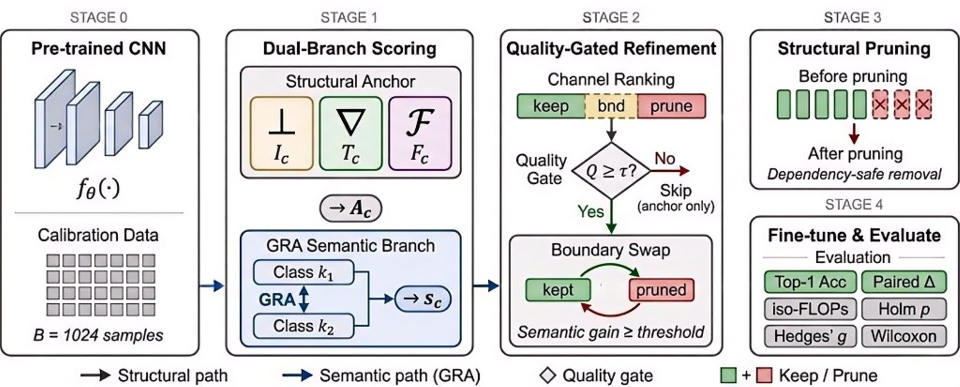
\includegraphics[width=\linewidth]{figures/fig_pipeline.pdf}
\caption{Workflow of GRA-CNN on image classification backbones.}
\label{fig:ivc_workflow}
\end{subfigure}\hfill
\begin{subfigure}[t]{0.54\textwidth}
\centering
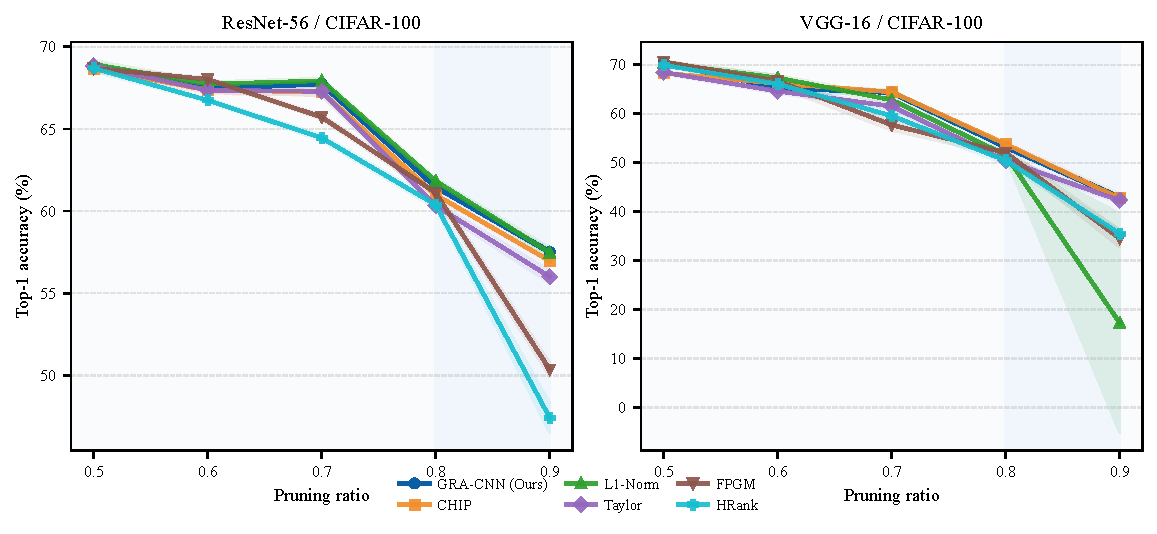
\includegraphics[width=\linewidth]{figures/fig_main_ratio_curves.pdf}
\caption{Five-ratio CIFAR-100 comparison on ResNet-56 and VGG-16.}
\label{fig:ivc_main_ratio_curves}
\end{subfigure}
\caption{Primary view of the method and the main CIFAR-100 trend. (a) GRA-CNN combines a structural anchor with class-aware GRA-based boundary refinement before dependency-safe pruning and recovery. (b) GRA-CNN becomes more competitive as compression increases, with the clearest separation appearing in residual high-compression cells.}
\label{fig:ivc_primary_pair}
\end{figure}

The five-ratio curves clarify why a robustness-centered interpretation is more appropriate than a universal-best interpretation. On ResNet-56, GRA-CNN remains especially competitive in the stressed regime, while at lower compression the gap among strong structural baselines is small. On VGG-16, method ordering changes more sharply with the operating point, which cautions against treating a single pruning score as architecture-agnostic.
\FloatBarrier

\subsection{Paired robustness and equal-budget evaluation}

The main paired comparison in Table~\ref{tab:robustness_budget_ivc} (left block) focuses on the residual cells that drive the paper's strongest claim. GRA-CNN shows positive paired deltas over CHIP at both $p=0.7$ and $p=0.9$, with Holm-adjusted significance in both cells. Against L1, the comparison is more nuanced: L1 remains strong at moderate compression, but it does not dominate consistently once robustness is considered across the full evaluation.

Raw pruning-ratio comparisons can be misleading when competing methods achieve different FLOPs. Table~\ref{tab:robustness_budget_ivc} (right block) therefore reports the iso-FLOPs results. Under matched budgets, the ResNet-56 advantage at $p=0.7$ remains positive, while the $p=0.9$ gap narrows. On VGG-16, GRA-CNN shows favorable directionality under equal budgets, even though the main-matrix advantage is modest. These matched-budget results support a restrained conclusion: the semantic branch is most convincing as a robustness-oriented complement when structural rankings become less stable.

\begin{table}[!htbp]
\caption{CIFAR-100 robustness-oriented statistical summaries. (a) Primary paired robustness statistics on ResNet-56 for the residual high-compression cells. (b) Iso-FLOPs comparison under matched computational budgets, with CHIP used as the reference within each cell.}
\label{tab:robustness_budget_ivc}
\centering
\begin{minipage}[t]{0.98\textwidth}
\centering
\textbf{(a) Paired robustness statistics}\par\medskip
\footnotesize
\setlength{\tabcolsep}{3pt}
\begin{tabular}{lccccc}
\toprule
Baseline & Ratio & $\Delta$ & 95\% CI & Holm $p$ & $g$ \\
\midrule
CHIP & 0.7 & +0.51 & [+0.42, +0.60] & 0.0037 & +3.50 \\
CHIP & 0.9 & +0.54 & [+0.40, +0.66] & 0.0100 & +2.56 \\
L1 & 0.7 & -0.17 & [-0.38, -0.01] & 0.3605 & -0.58 \\
L1 & 0.9 & +0.04 & [-0.15, +0.21] & 0.7452 & +0.12 \\
\bottomrule
\end{tabular}
\end{minipage}

\vspace{0.8em}

\begin{minipage}[t]{0.98\textwidth}
\centering
\textbf{(b) Iso-FLOPs comparison}\par\medskip
\footnotesize
\setlength{\tabcolsep}{3pt}
\begin{tabular}{llccccc}
\toprule
Architecture & Ratio & CHIP & GRA-CNN & L1 & $\Delta_G$ & $\Delta_L$ \\
\midrule
ResNet-56 & 0.7 & 64.64 & 65.52 & \textbf{65.93} & +0.88 & +1.29 \\
ResNet-56 & 0.9 & \textbf{51.19} & 50.97 & 50.41 & -0.22 & -0.78 \\
VGG-16 & 0.7 & 63.64 & \textbf{64.26} & 57.64 & +0.62 & -6.00 \\
VGG-16 & 0.9 & 39.30 & \textbf{42.55} & 30.43 & +3.26 & -8.86 \\
\bottomrule
\end{tabular}
\end{minipage}
\end{table}

\FloatBarrier

\subsection{Component contribution and semantic evidence}

Table~\ref{tab:ablation_summary_ivc} and Figure~\ref{fig:ivc_mechanism_pair} show that all three components of GRA-CNN matter: channel attention, boundary refinement, and quality gating. Every component removal reduces accuracy, and the penalties grow under aggressive compression. Figure~\ref{fig:ivc_mechanism_pair}(b) provides mechanism-level support for the semantic interpretation. GRA and L1 rankings show weak correlation on a representative layer, and the visualized channel responses suggest that GRA prioritizes more class-relevant localized patterns than a purely structural score. We use this view as supporting evidence for the semantic mechanism, not as standalone causal proof.

\begin{table}[!htbp]
\centering
\begin{minipage}[t]{0.62\textwidth}
\captionsetup{type=table}
\caption{Component ablation summary on ResNet-56 and VGG-16 at $p=0.7$ and $p=0.9$. Values are mean$\pm$std Top-1 accuracy over five seeds.}
\label{tab:ablation_summary_ivc}
\scriptsize
\resizebox{\linewidth}{!}{%
\begin{tabular}{llcccc}
\toprule
Architecture & Ratio & Full & w/o CA & w/o Boundary & w/o Gate \\
\midrule
ResNet-56 & $p=0.7$ & \textbf{67.76$\pm$0.17} & 65.59$\pm$0.28 & 65.71$\pm$0.10 & 66.02$\pm$0.11 \\
ResNet-56 & $p=0.9$ & \textbf{57.51$\pm$0.16} & 51.46$\pm$0.23 & 51.62$\pm$0.16 & 51.70$\pm$0.41 \\
VGG-16 & $p=0.7$ & \textbf{64.37$\pm$0.35} & 61.36$\pm$0.33 & 61.68$\pm$0.22 & 61.73$\pm$0.17 \\
VGG-16 & $p=0.9$ & \textbf{42.84$\pm$0.40} & 35.53$\pm$0.61 & 36.11$\pm$0.28 & 33.83$\pm$1.75 \\
\bottomrule
\end{tabular}
}
\end{minipage}\hfill
\begin{minipage}[t]{0.34\textwidth}
\captionsetup{type=table}
\caption{Auxiliary similarity-metric sensitivity on ResNet-56/CIFAR-100 under the matched five-seed, 40-epoch recovery protocol.}
\label{tab:metric_sensitivity_ivc}
\scriptsize
\resizebox{\linewidth}{!}{%
\begin{tabular}{lcc}
\toprule
Method & $p=0.7$ & $p=0.9$ \\
\midrule
GRA-CNN & 66.16$\pm$0.23 & 54.27$\pm$0.44 \\
Cosine-Semantic & 65.99$\pm$0.18 & 54.54$\pm$0.53 \\
Correlation-Semantic & 65.93$\pm$0.18 & 52.15$\pm$1.25 \\
\bottomrule
\end{tabular}
}
\vspace{0.2em}

\footnotesize
GRA-CNN vs.\ Cosine-Semantic: n.s.\\
GRA-CNN vs.\ Correlation-Semantic at $p=0.9$: +2.12 pp ($p=0.045$).
\end{minipage}
\end{table}


\begin{figure}[!htbp]
\centering
\begin{subfigure}[t]{0.58\textwidth}
\centering
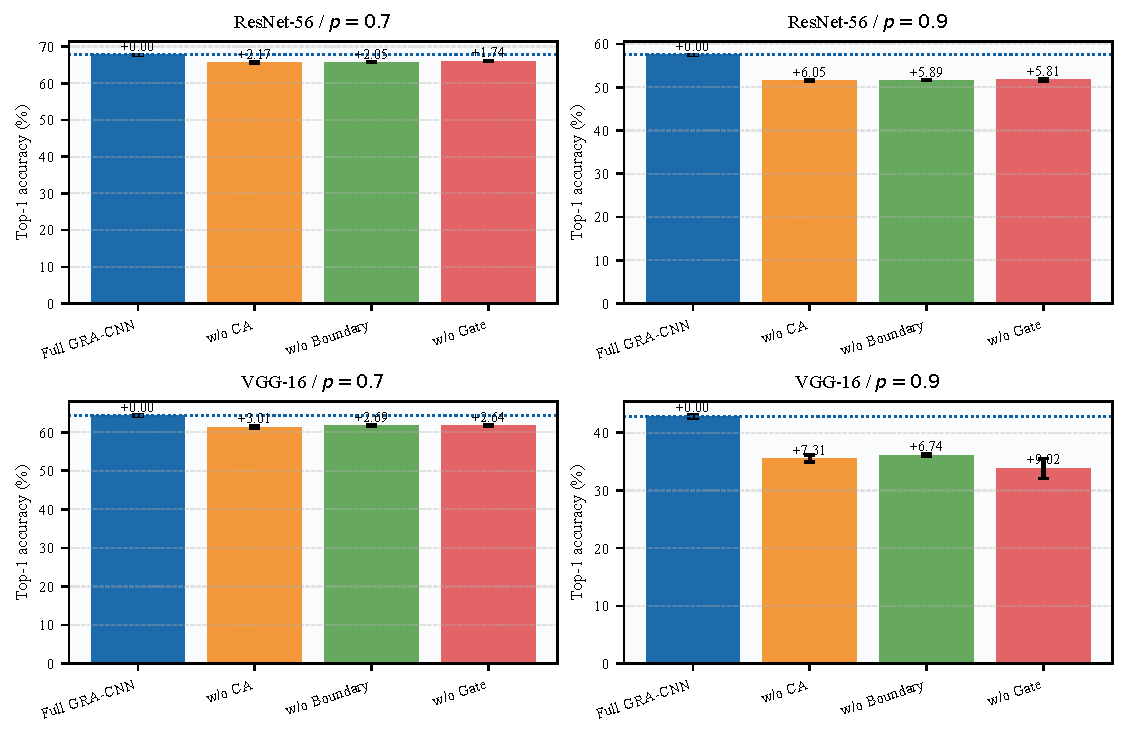
\includegraphics[width=\linewidth]{figures/fig_ablation_extended.pdf}
\caption{Extended multi-seed ablation on ResNet-56 and VGG-16 at $p=0.7$ and $p=0.9$.}
\label{fig:ivc_ablation}
\end{subfigure}\hfill
\begin{subfigure}[t]{0.38\textwidth}
\centering
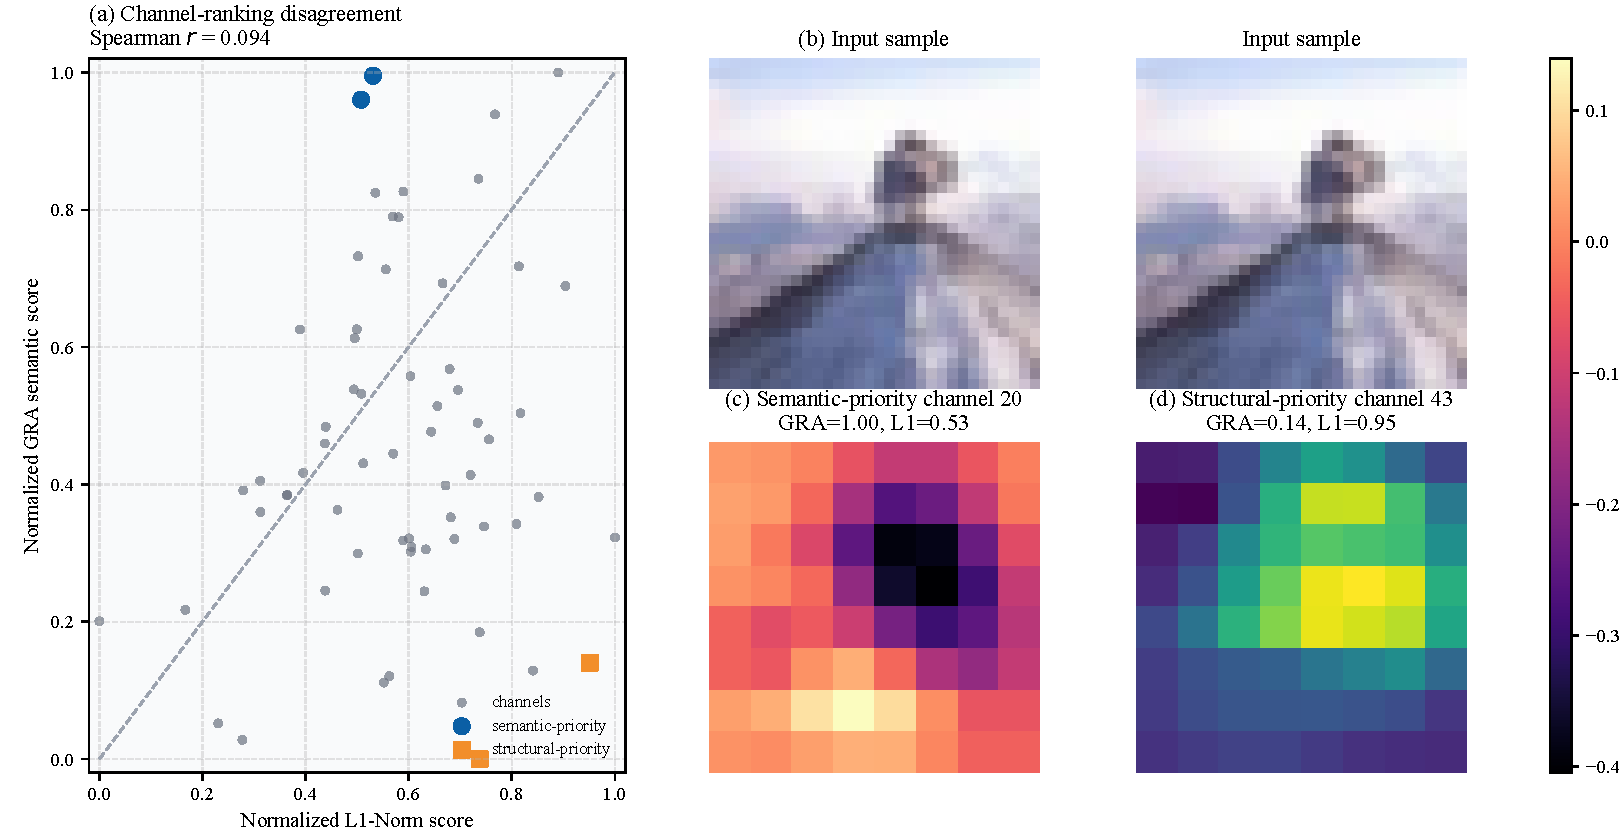
\includegraphics[width=\linewidth]{figures/fig_semantic_evidence.pdf}
\caption{Mechanism-level semantic evidence on ResNet-56/CIFAR-100.}
\label{fig:ivc_semantic_evidence}
\end{subfigure}
\caption{Mechanism validation of GRA-CNN. (a) Removing any component degrades performance, with the largest penalties appearing under aggressive compression. (b) GRA and L1 rank channels differently, and the highlighted response maps suggest that GRA better preserves class-relevant localized behavior.}
\label{fig:ivc_mechanism_pair}
\end{figure}
\FloatBarrier

\subsection{Similarity metric sensitivity}

To test whether the observed gain depends specifically on Gray Relational Analysis or more broadly on the semantic-refinement framework, we ran an auxiliary metric ablation on ResNet-56/CIFAR-100 in which the semantic branch was kept intact but the similarity score was replaced by cosine similarity or Pearson correlation. This auxiliary study used the same five seeds but a separate 40-epoch recovery protocol, so it is reported alongside, rather than merged into, the main 30-epoch matrix.

Cosine-Semantic remained close to the GRA-CNN baseline at both ratios, with no significant difference in either case (Table~\ref{tab:metric_sensitivity_ivc}). Correlation-Semantic behaved similarly at $p=0.7$ but degraded at $p=0.9$, where GRA-CNN retained a +2.12 pp advantage (paired $p=0.045$). This result suggests that the main contribution is better understood as the semantic refinement framework and its quality-gated boundary use, rather than the claim that GRA is the only workable similarity metric. At the same time, the correlation replacement is less stable under aggressive compression, which supports retaining GRA as the default metric in the proposed method.
\FloatBarrier

\subsection{Transfer robustness on Tiny-ImageNet}

\begin{figure}[!htbp]
\centering
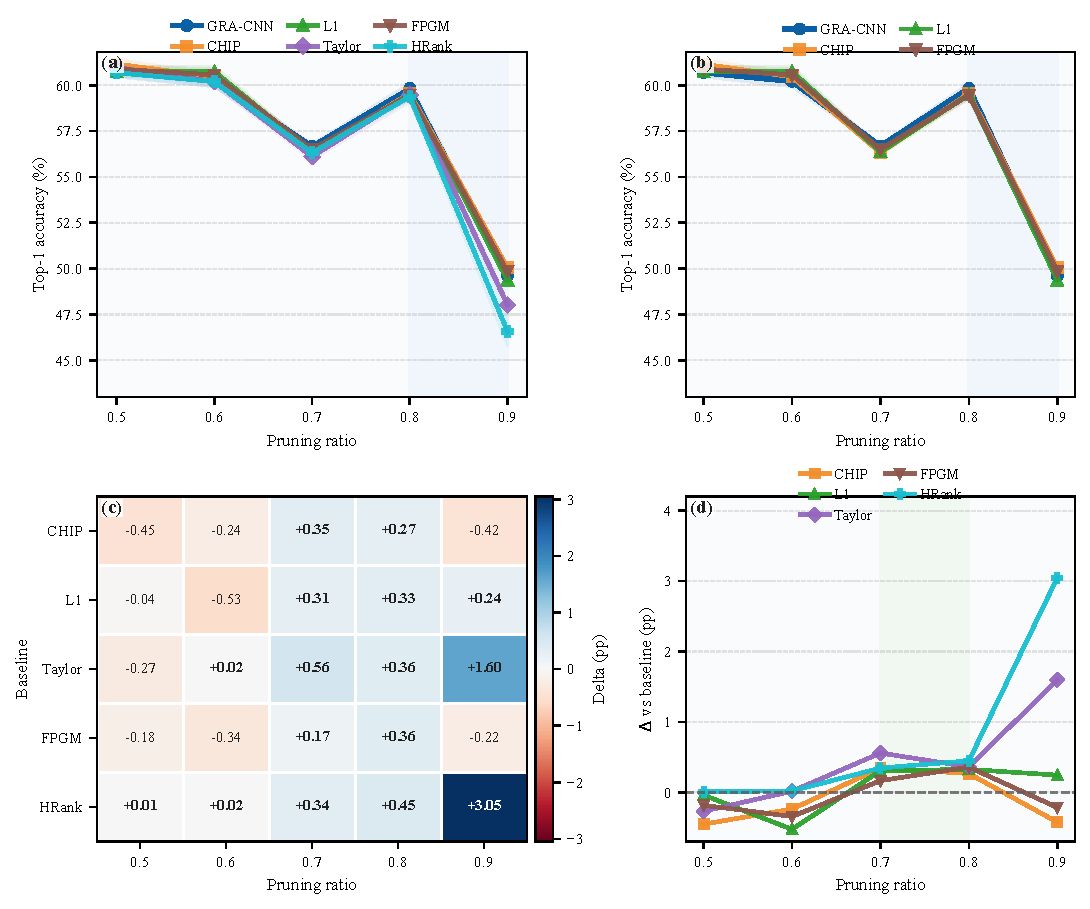
\includegraphics[width=0.95\linewidth]{figures/fig_tiny_matrix.pdf}
\caption{Formal five-ratio, five-seed Tiny-ImageNet transfer study on ResNet-18. Panels (a) and (b) show the full sweep and the frontier-focused view. Panels (c) and (d) summarize paired deltas against the baselines and make the moderate-to-high compression advantage easier to read.}
\label{fig:ivc_tiny_pair}
\end{figure}

Figure~\ref{fig:ivc_tiny_pair} summarizes the full five-ratio transfer sweep on ResNet-18/Tiny-ImageNet. The five-point curve sharpens the regime-dependent interpretation. At low compression, GRA-CNN is not uniformly dominant: it trails CHIP by 0.45 pp at $p=0.5$ and remains nearly tied with the strongest baselines at $p=0.6$. The most favorable region appears at moderate-to-high compression. At $p=0.7$, GRA-CNN is the best method and exceeds CHIP, L1, Taylor, FPGM, and HRank by +0.35, +0.31, +0.56, +0.17, and +0.34 pp, respectively. At $p=0.8$, it again ranks first, although the margins are modest and the cell remains closer to a near-tie than to clear separation. At the most aggressive endpoint ($p=0.9$), GRA-CNN remains better than L1, Taylor, and HRank but trails CHIP and FPGM slightly. The frontier view in panel (b) and the delta summaries in panels (c) and (d) make the operating-region pattern easier to read: the semantic refinement is most favorable around $p=0.7$--$0.8$, while the low-compression cells remain near-tied and the $p=0.9$ endpoint becomes mixed.
\FloatBarrier

\subsection{Robustness across compression ratios and scoring sensitivity}

Figure~\ref{fig:ivc_robustness_pair} summarizes two robustness-oriented supporting views. Figure~\ref{fig:ivc_robustness_pair}(a) restores the dense-ratio sweep to the main paper. On ResNet-56, GRA-CNN remains most competitive in the stressed residual region and stays near strong baselines elsewhere. On VGG-16, the same sweep is more volatile, which reinforces the paper's architecture-dependent interpretation. Figure~\ref{fig:ivc_robustness_pair}(b) summarizes the multi-seed sensitivity study over the distinguishing coefficient and calibration size. The dominant message is stability rather than aggressive tuning sensitivity: the default configuration remains close to the best-performing region, and the main conclusions do not depend on narrow hyperparameter choices. This matters for practical use because a semantic refinement branch would be less convincing if its gains were driven by fragile tuning.

\begin{figure}[!htbp]
\centering
\begin{subfigure}[t]{0.50\textwidth}
\centering
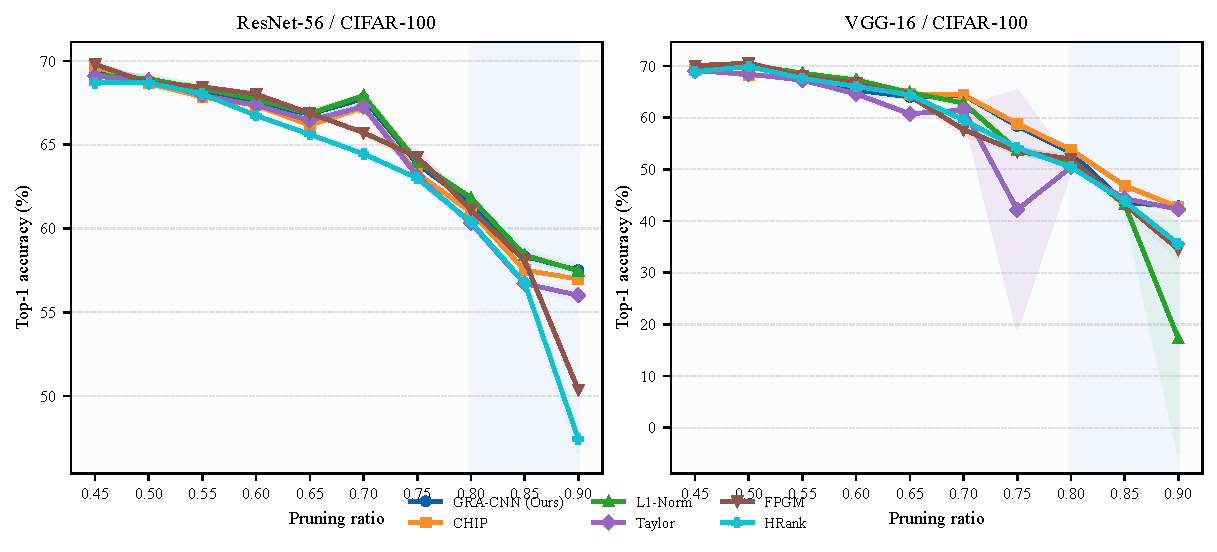
\includegraphics[width=\linewidth]{figures/fig_dense_ratio_extension.pdf}
\caption{Dense pruning-ratio extension on CIFAR-100.}
\label{fig:ivc_dense_ratio_extension}
\end{subfigure}\hfill
\begin{subfigure}[t]{0.46\textwidth}
\centering
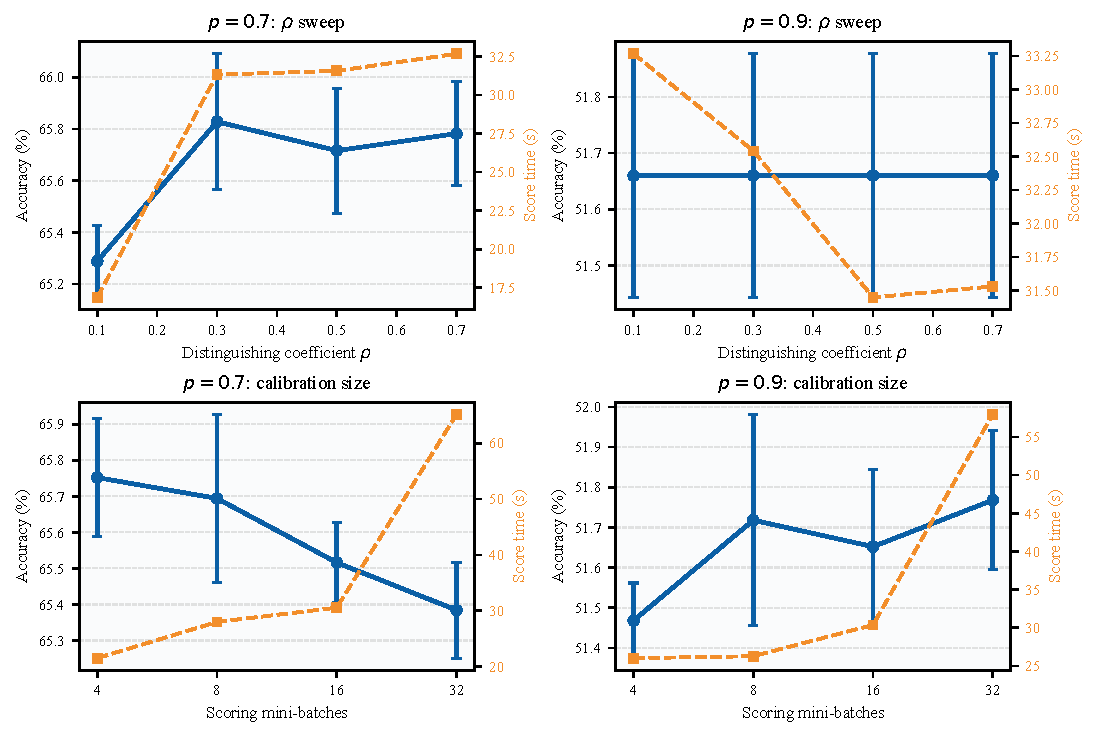
\includegraphics[width=\linewidth]{figures/fig_sensitivity_multiregime.pdf}
\caption{Multi-regime sensitivity on ResNet-56/CIFAR-100.}
\label{fig:ivc_sensitivity_multiregime}
\end{subfigure}
\caption{Robustness-oriented supporting evidence. (a) Across dense ratios, the residual-network trend is more favorable to GRA-CNN in the high-compression region than the corresponding VGG-16 trend. (b) The default semantic-scoring configuration remains near a stable operating region.}
\label{fig:ivc_robustness_pair}
\end{figure}

The full paired Tiny-ImageNet table and secondary diagnostics remain in the Supplementary Material together with runtime and latency analyses. This keeps the main paper visually fuller while preserving the complete evidence chain for reproducibility.
\FloatBarrier

\section{Discussion and Limitations}
\label{sec:discussion}

The results support a narrower and, in our view, more credible claim than ``best method everywhere''. GRA-CNN is most effective when structural-only rankings become brittle, especially in high-compression residual CNNs. On ResNet-56, this appears in both the raw accuracy comparisons and the paired statistics. On VGG-16, the method shows directionally positive behavior under matched budgets, but the gains are less stable. The architecture dependence is therefore part of the empirical story, not an afterthought.

The observed architecture sensitivity likely stems from differences in feature redundancy patterns. Residual networks with skip connections naturally distribute information across multiple paths, making class-aware redundancy analysis more informative when deciding which channels to prune. In contrast, plain feed-forward architectures like VGG may exhibit more uniform channel importance distributions, reducing the relative advantage of semantic refinement over structural heuristics. This suggests that the benefit of class-conditioned scoring is not universal but rather depends on the architectural inductive bias and the degree to which channels specialize for different semantic patterns.

This robustness-oriented interpretation is reinforced by the ablation study. Even in cells where the net gain over CHIP is small, removing channel attention, boundary refinement, or quality gating causes noticeable degradation. The dense-ratio figure shows that the favorable region is concentrated rather than random. The sensitivity figure indicates that the same region does not depend on fragile hyperparameter tuning. Taken together, the results support viewing the method as a semantic correction mechanism. Its benefit depends on uncertainty in the structural ranking.

The quality gating mechanism plays a critical role in preventing semantic scoring from being applied indiscriminately. In layers where the structural anchor and semantic scores disagree strongly, or where semantic dispersion is low, forcing semantic refinement can introduce instability. The gating threshold adaptively identifies layers where the semantic signal is sufficiently reliable, effectively turning GRA into a targeted intervention rather than a blanket replacement. This design choice reflects a practical trade-off: semantic scoring is computationally more expensive than structural heuristics, so it should be reserved for cases where it provides clear added value.

Another practical implication is that pruning quality should be interpreted as a regime-level property rather than as a single operating-point score. In our experiments, paired statistics, matched-budget comparisons, and cross-dataset transfer checks helped distinguish stable behavior from isolated wins. This matters in structured pruning because small nominal accuracy gaps can disappear once FLOPs are matched or the pruning ratio changes. The proposed framework is therefore useful not only as a pruning strategy, but also as a disciplined evaluation setting for identifying when semantic correction is genuinely beneficial.

The study also has clear limitations. The primary benchmarks are still CIFAR-100 and Tiny-ImageNet rather than ImageNet-scale classification or downstream dense prediction tasks. The strongest results remain concentrated in residual CNNs, so the conclusions should not be extrapolated to all architectures. The metric-sensitivity study also indicates that part of the benefit comes from the overall semantic refinement framework rather than from an exclusive dependence on one similarity definition. Device-level latency profiling is provided only on a single RTX 5090 platform and is therefore informative but not exhaustive. Finally, although five-seed statistics improve reliability relative to single-run reporting, larger seed pools would further strengthen the smallest observed effects.

Additional limitations include the restriction to image classification tasks, whereas structured pruning is increasingly important for object detection, semantic segmentation, and video understanding where computational constraints are even more critical. The calibration set size and composition may also influence the reliability of class-aware redundancy estimates, particularly for datasets with severe class imbalance or fine-grained visual categories. The current gating mechanism uses fixed percentile thresholds that were tuned on CIFAR-100; adaptive threshold selection based on dataset statistics could improve generalization to other domains. Furthermore, the interaction between GRA-CNN and other compression techniques such as quantization, knowledge distillation, or neural architecture search remains unexplored and could reveal synergies or conflicts that affect deployment viability.

\section{Conclusion}
\label{sec:conclusion}

We presented GRA-CNN, a semantic-aware structured pruning framework. It uses a structural anchor together with quality-gated Gray Relational Analysis at the keep/prune boundary. The method is designed as a robustness-oriented refinement, not as a universal end-to-end scorer. Across the multi-seed CIFAR-100 experiments, matched-budget comparisons, component ablations, a similarity-metric sensitivity study, and a five-ratio Tiny-ImageNet transfer sweep, GRA-CNN shows its clearest benefits in high-compression residual CNN settings. It remains directionally positive elsewhere.

The main takeaway is therefore pragmatic: class-aware semantic redundancy can improve structured pruning robustness when structural-only rankings are under stress. The auxiliary metric ablation further suggests that the main contribution lies in the semantic refinement framework and its gated boundary use, while GRA remains a stable default under aggressive compression. This makes GRA-CNN a useful addition to the pruning toolbox for visual models, especially in regimes where compression is aggressive and reliability matters more than isolated best-case scores.

Future work could extend this framework to larger-scale datasets such as full ImageNet, explore its applicability to vision transformers where attention mechanisms may interact differently with class-aware redundancy, and investigate adaptive gating strategies that dynamically adjust the semantic refinement intensity based on layer-wise uncertainty estimates. Additionally, combining GRA-CNN with neural architecture search or knowledge distillation could further improve the trade-off between compression and accuracy in deployment-critical scenarios.

\section*{Declaration of competing interest}
The authors declare that they have no known competing financial interests or personal relationships that could have appeared to influence the work reported in this paper.

\section*{Funding}
This research received no external funding.

\section*{CRediT authorship contribution statement}
Kangrui Li: Software, formal analysis, visualization, writing - original draft. Junyi Lin: Validation, investigation, writing - review and editing. Xiaobo Zhang: Conceptualization, methodology, supervision, writing - review and editing.

\section*{Data availability}
The datasets used in this study are publicly available benchmarks. Run-level JSON records, tabulated results, and figure-generation scripts are available in the project repository.\\
\url{https://github.com/Deepmind666/GRA-CNN}

\section*{Supplementary material}
Supplementary material associated with this article includes the full five-ratio CIFAR-100 matrix, the full Tiny-ImageNet transfer table, runtime and latency profiles, dense-ratio diagnostics, and multi-seed sensitivity analyses.

\section*{Declaration of generative AI and AI-assisted technologies in the writing process}
During the preparation of this work, the authors used generative AI tools to assist with language polishing, structural editing, and formatting. After using these tools, the authors reviewed and edited the content as needed and take full responsibility for the final content of the publication.

\bibliographystyle{elsarticle-num}
\bibliography{references}

\end{document}
